% CH4114 — Tutorial 00, Part 2: Organizing Your Project
% Beamer deck, 16:9, compiled with pdflatex (TeX Live 2026)
\documentclass[aspectratio=169]{beamer}

\usetheme{Madrid}
\usecolortheme{whale}
\setbeamertemplate{navigation symbols}{}

\usepackage[T1]{fontenc}
\usepackage{tikz}
\usetikzlibrary{arrows.meta, positioning}
\usepackage{booktabs}
\usepackage{listings}
\lstset{
  basicstyle=\ttfamily\footnotesize,
  breaklines=true,
  showstringspaces=false,
  columns=fullflexible,
  keepspaces=true,
}

\title[Project Organization]{Tutorial 00 --- Part 2\\[2pt] Organizing Your Project}
\subtitle{The professional Python folder layout}
\author[S. B. Seal]{Shuvam Banerji Seal}
\institute[CH4114]{CH4114 --- Molecular Simulation}
\date[Aug 2026]{14 August 2026}

\begin{document}

% ------------------------------------------------------------------ title
\begin{frame}[plain]
  \titlepage
  \centering{\scriptsize Repository: \texttt{CH4114\_Molecular\_Simulation\_Tutorials}}
\end{frame}

% ------------------------------------------------------------ why matters
\begin{frame}{Why folder structure matters}
  \begin{columns}[T]
    \begin{column}{0.44\textwidth}
      \begin{itemize}
        \item One week in, a flat folder becomes unsearchable.
        \item ``Which script made this figure?'' must be answerable.
        \item Structure is how a team (or future-you) communicates.
      \end{itemize}
    \end{column}
    \begin{column}{0.52\textwidth}
      \begin{center}
        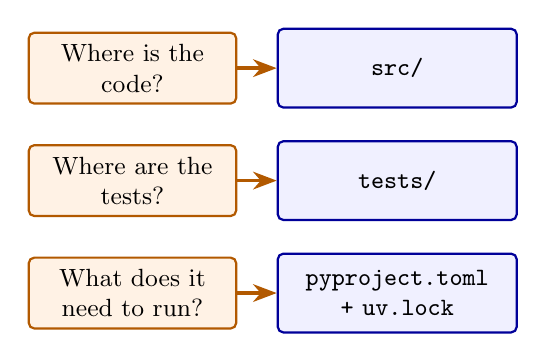
\begin{tikzpicture}[
            q/.style={rectangle, draw=orange!70!black, thick, rounded corners=2pt,
                      fill=orange!10, text width=2.4cm, align=center,
                      minimum height=0.9cm, font=\small},
            a/.style={rectangle, draw=blue!60!black, thick, rounded corners=2pt,
                      fill=blue!6, text width=2.8cm, align=center,
                      minimum height=1.0cm, font=\small},
            arr/.style={-{Stealth[length=3mm]}, very thick, orange!70!black},
            node distance=0.5cm]
          \node[q] (q1) {Where is the\\ code?};
          \node[q, below=of q1] (q2) {Where are the\\ tests?};
          \node[q, below=of q2] (q3) {What does it\\ need to run?};
          \node[a, right=0.5cm of q1] (a1) {\texttt{src/}};
          \node[a, right=0.5cm of q2] (a2) {\texttt{tests/}};
          \node[a, right=0.5cm of q3] (a3) {\texttt{pyproject.toml}\\ \texttt{+ uv.lock}};
          \draw[arr] (q1) -- (a1);
          \draw[arr] (q2) -- (a2);
          \draw[arr] (q3) -- (a3);
        \end{tikzpicture}
      \end{center}
    \end{column}
  \end{columns}
  \vspace{0.2cm}
  \begin{block}{Three questions a good layout answers instantly}
    Code $\rightarrow$ \texttt{src/} \enspace$\cdot$\enspace Tests $\rightarrow$ \texttt{tests/}\\
    Dependencies $\rightarrow$ \texttt{pyproject.toml} + \texttt{uv.lock}
  \end{block}
\end{frame}

% ---------------------------------------------------------- canonical layout
\begin{frame}[fragile]{The canonical layout}
  \begin{columns}[T]
    \begin{column}{0.5\textwidth}
      \begin{lstlisting}[basicstyle=\ttfamily\scriptsize]
my_project/
+-- README.md
+-- LICENSE
+-- pyproject.toml
+-- uv.lock
+-- .gitignore
+-- .python-version
+-- src/
|   +-- my_project/
|       +-- __init__.py
|       +-- potentials.py
|       +-- analysis.py
+-- tests/
|   +-- test_potentials.py
+-- docs/
+-- scripts/
+-- assets/
+-- notebooks/
      \end{lstlisting}
    \end{column}
    \begin{column}{0.46\textwidth}
      \begin{itemize}
        \item \textbf{README} --- the front page: what, why, how to run.
        \item \textbf{pyproject.toml} --- single source of truth for metadata
              and dependencies.
        \item \textbf{uv.lock} --- machine-generated; commit it.
        \item \textbf{.gitignore} --- keep \texttt{.venv/}, caches, secrets out.
        \item \textbf{src/} --- the importable package.
        \item \textbf{tests/} --- verification, outside the package.
      \end{itemize}
    \end{column}
  \end{columns}
\end{frame}

% -------------------------------------------------------------- src-layout
\begin{frame}{Why the src-layout?}
  \begin{center}
    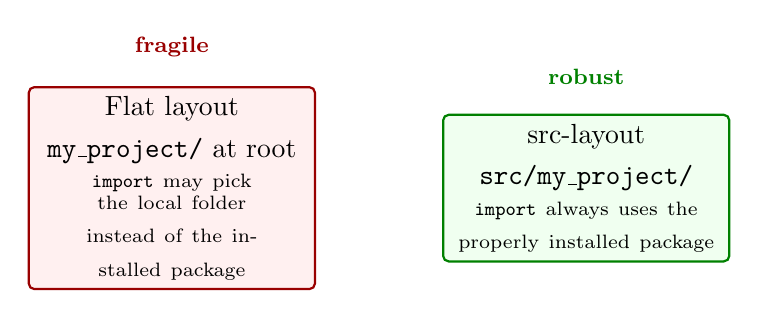
\begin{tikzpicture}[
        flat/.style={rectangle, draw=red!60!black, thick, rounded corners=2pt,
                     fill=red!6, text width=3.4cm, align=center,
                     minimum height=1.6cm},
        src/.style={rectangle, draw=green!50!black, thick, rounded corners=2pt,
                    fill=green!6, text width=3.4cm, align=center,
                    minimum height=1.6cm},
        node distance=1.6cm]
      \node[flat] (f) {Flat layout\\[3pt] \texttt{my\_project/} at root\\[3pt]
                       {\scriptsize \texttt{import} may pick the local folder\\ instead of the installed package}};
      \node[src, right=of f] (s) {src-layout\\[3pt] \texttt{src/my\_project/}\\[3pt]
                       {\scriptsize \texttt{import} always uses the\\ properly installed package}};
      \node[above=0.25cm of f, font=\footnotesize\bfseries, text=red!60!black] {fragile};
      \node[above=0.25cm of s, font=\footnotesize\bfseries, text=green!50!black] {robust};
    \end{tikzpicture}
  \end{center}
  \vspace{0.3cm}
  \begin{itemize}
    \item Prevents the classic bug: tests pass locally, fail elsewhere.
    \item The layout used by most modern Python projects --- and this repo.
  \end{itemize}
\end{frame}

% ------------------------------------------------------------ file contracts
\begin{frame}{What each file promises}
  \begin{table}
    \small
    \begin{tabular}{@{}ll@{}}
      \toprule
      File & Contract \\
      \midrule
      \texttt{README.md} & 30-second explanation: what, why, how to run \\
      \texttt{pyproject.toml} & single source of truth: name, version, Python, deps \\
      \texttt{uv.lock} & machine-generated; pins every transitive dependency \\
      \texttt{.gitignore} & never commit \texttt{.venv/}, caches, secrets \\
      \texttt{LICENSE} & who may use it, under what terms \\
      \texttt{src/<pkg>/\_\_init\_\_.py} & marks the package; often holds version \\
      \bottomrule
    \end{tabular}
  \end{table}
  \vspace{0.3cm}
  \begin{block}{Rule of thumb}
    Generated files $\rightarrow$ out of Git. Files needed to \emph{reproduce}
    the project $\rightarrow$ in Git.
  \end{block}
\end{frame}

% ------------------------------------------------------------ conventions
\begin{frame}{Naming conventions: be consistent}
  \begin{table}
    \small
    \begin{tabular}{@{}lll@{}}
      \toprule
      Thing & Convention & Example \\
      \midrule
      Repositories & kebab/snake & \texttt{CH4114\_Molecular\_Simulation\_Tutorials} \\
      Python packages & snake & \texttt{ch4114}, \texttt{mdtraj} \\
      Python files & snake & \texttt{lj\_potential.py} \\
      Test files & \texttt{test\_<module>.py} & \texttt{test\_lj\_potential.py} \\
      Branches & kebab & \texttt{fix-neighbor-list} \\
      Tutorial folders & \texttt{tutorial\_<NN>\_<DD-MM-YYYY>} & \texttt{tutorial\_00\_14-08-2026} \\
      \bottomrule
    \end{tabular}
  \end{table}
  \vspace{0.3cm}
  \begin{block}{Commit messages}
    \texttt{feat: add Lennard-Jones potential module} \\
    \texttt{fix: correct prefactor in Ewald summation} \\
    \texttt{docs: explain thermostat choice in README} \\
    \texttt{test: cover neighbor-list edge cases}
  \end{block}
\end{frame}

% ------------------------------------------------------------ sim example
\begin{frame}[fragile]{A simulation-specific example}
  \begin{columns}[T]
    \begin{column}{0.55\textwidth}
      \begin{lstlisting}[basicstyle=\ttfamily\scriptsize]
md_project/
+-- README.md
+-- pyproject.toml
+-- uv.lock
+-- src/md_project/
|   +-- potentials.py
|   +-- integrators.py
|   +-- ensembles.py
|   +-- io.py
+-- tests/
|   +-- test_potentials.py
|   +-- test_integrators.py
+-- scripts/
|   +-- run_benchmark.py
+-- docs/
|   +-- methodology.md
+-- assets/figures/
      \end{lstlisting}
    \end{column}
    \begin{column}{0.42\textwidth}
      \begin{itemize}
        \item Code: LJ, Coulomb, Verlet, thermostats.
        \item Tests verify physics, not just syntax.
        \item \texttt{scripts/} for one-off benchmarks.
        \item \texttt{docs/methodology.md} --- write down what you did and why.
        \item Data and figures are \textbf{regenerated}, not committed.
      \end{itemize}
    \end{column}
  \end{columns}
\end{frame}

% ------------------------------------------------------------ anti-patterns
\begin{frame}{Anti-patterns to avoid}
  \begin{table}
    \small
    \begin{tabular}{@{}ll@{}}
      \toprule
      Anti-pattern & Why it hurts \\
      \midrule
      \texttt{analysis\_final\_v2\_really.py} & version control exists --- use it \\
      Everything in one folder & nobody can find anything \\
      Committing \texttt{.venv/} & huge, machine-specific, breaks everyone \\
      No README & the repo is a black box \\
      \texttt{pip freeze $>$ requirements.txt} & pins your whole machine, not the project \\
      Editing \texttt{main} directly & no review, no record of intent \\
      \bottomrule
    \end{tabular}
  \end{table}
\end{frame}

% ------------------------------------------------------------ check yourself
\begin{frame}{Check yourself}
  \begin{enumerate}
    \item Why does the package live under \texttt{src/} instead of the repo root?
    \item Which three files answer ``what does this project need to run?''?
    \item Name two things that must never be committed to Git.
    \item What is the tutorial folder naming convention?
  \end{enumerate}
  \vspace{0.4cm}
  \begin{block}{Next up}
    Part 3: uv --- Python environments without the pain.
  \end{block}
\end{frame}

\end{document}
